\section{Transformation of Nonlinear Equations into Separable Equations}

\noindent
In Section~2.1 we found that the solutions of a linear nonhomogeneous equation
\[
  y'+p(x)y=f(x)
\]
are of the form $y=uy_{1}$, where $y_{1}$ is a nontrivial solution of the complementary equation
\begin{equation}
  \label{eq:2.4.1}y'+p(x)y=0
\end{equation}
and $u$ is a solution of
\[
  u'y_{1}(x)=f(x).
\]
Note that this last equation is separable, since it can be rewritten as
\[
  u'=\frac{f(x)}{y_{1}(x)}.
\]
In this section we'll consider nonlinear differential equations that are not separable to begin with, but can be solved in a similar fashion by writing their solutions in the form $y=uy_{1}$, where $y_{1}$ is a suitably chosen known function and $u$ satisfies a separable equation. We'll say in this case that we {\color{blue}\it transformed\/} the given equation into a separable equation.

\boxit{Bernoulli Equations}

\noindent
A
\href{https://mathshistory.st-andrews.ac.uk/Biographies/Bernoulli_Jacob/}{\color{blue}
\it Bernoulli equation}
is an equation of the form
\begin{equation}
  \label{eq:2.4.2}y'+p(x)y=f(x)y^{r},
\end{equation}
where $r$ can be any real number other than $0$ or $1$. (Note that \eqref{eq:2.4.2} is linear if and only if $r=0$ or $r=1$.) We can transform \eqref{eq:2.4.2} into a separable equation by variation of parameters: if $y_{1}$ is a nontrivial solution of \eqref{eq:2.4.1}, substituting $y=uy_{1}$ into \eqref{eq:2.4.2} yields
\[
  u'y_{1}+u(y_{1}'+p(x)y_{1})=f(x)(uy_{1})^{r},
\]
which is equivalent to the separable equation
\[
  u'y_{1}(x)=f(x)\left(y_{1}(x)\right)^{r}u^{r}\mbox{\quad or \quad}{\frac{u'}{u^{r}}}=f(x)\left(y_{1}(x)\right)^{r-1},
\]
since $y_{1}'+p(x)y_{1}=0$.

\begin{example}
  \label{example:2.4.1} \rm Solve the Bernoulli equation
  \begin{equation}
    \label{eq:2.4.3}y'-y=xy^{2}.
  \end{equation}
\end{example}

\solution Since $y_{1}=e^{x}$ is a solution of $y'-y=0$, we look for solutions of \eqref{eq:2.4.3} in the form $y=ue^{x}$, where
\[
  u'e^{x}=xu^{2}e^{2x}\mbox{\quad or, equivalently, \quad}u'=xu^{2}e^{x}.
\]
Separating variables yields
\[
  \frac{u'}{u^{2}}=xe^{x},
\]
and integrating yields
\[
  -\frac{1}{u}=(x-1)e^{x}+c.
\]
Hence,
\[
  u=-\frac{1}{(x-1)e^{x}+c}
\]
and
\[
  y=-\frac{1}{x-1+ce^{-x}}.
\]

Figure~\ref{eq:2.4.1} shows direction field and some integral curves of \eqref{eq:2.4.3}.

\begin{figure}[tbp]
  \centering
  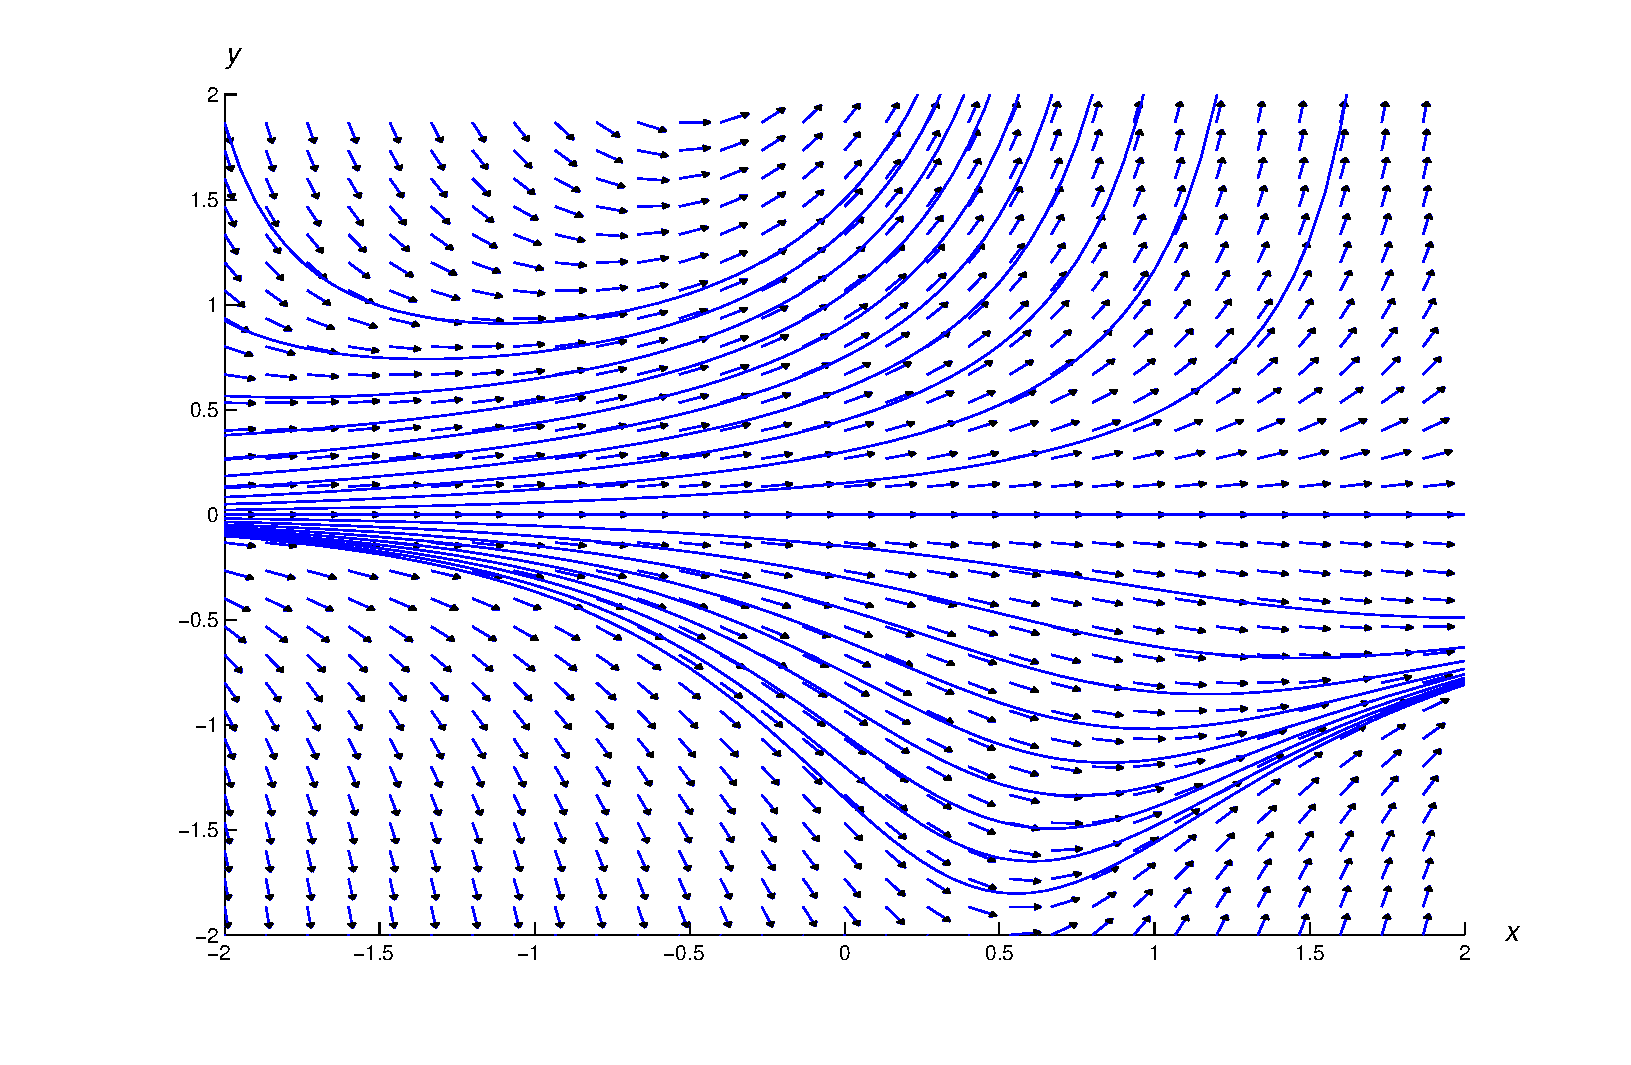
\includegraphics[bb=-78 148 689 643, width=5.67in, height=3.66in, keepaspectratio]{fig020401}
  \color{blue}
  \caption{A direction field and integral curves for $y'-y=xy^{2}$}
  \label{figure:2.4.1}
\end{figure}

\boxit{Other Nonlinear Equations That Can be Transformed Into Separable Equations}

\noindent
We've seen that the nonlinear Bernoulli equation can be transformed into a separable equation by the substitution $y=uy_{1}$ if $y_{1}$ is suitably chosen. Now let's discover a sufficient condition for a nonlinear first order differential equation
\begin{equation}
  \label{eq:2.4.4}y'=f(x,y)
\end{equation}
to be transformable into a separable equation in the same way. Substituting $y=uy_{1}$ into \eqref{eq:2.4.4} yields
\[
  u'y_{1}(x)+uy_{1}'(x)=f(x,uy_{1}(x)),
\]
which is equivalent to
\begin{equation}
  \label{eq:2.4.5}u'y_{1}(x)=f(x,uy_{1}(x))-uy_{1}'(x).
\end{equation}
If
\[
  f(x,uy_{1}(x))=q(u)y_{1}'(x)
\]
for some function $q$, then \eqref{eq:2.4.5} becomes
\begin{equation}
  \label{eq:2.4.6}u'y_{1}(x)=(q(u)-u)y_{1}'(x),
\end{equation}
which is separable. After checking for constant solutions $u\equiv u_{0}$ such that $q(u_{0})=u_{0}$, we can separate variables to obtain
\[
  \frac{u'}{q(u)-u}=\frac{y_{1}'(x)}{y_{1}(x)}.
\]

\boxit{Homogeneous Nonlinear Equations}

\noindent
In the text we'll consider only the most widely studied class of equations for which the method of the preceding paragraph works. Other types of equations appear in Exercises~\ref{exer:2.4.44}--\ref{exer:2.4.51}.

The differential equation \eqref{eq:2.4.4} is said to be {\color{blue}\it homogeneous\/} if $x$ and $y$ occur in $f$ in such a way that $f(x,y)$ depends only on the ratio $y/x$; that is, \eqref{eq:2.4.4} can be written as
\begin{equation}
  \label{eq:2.4.7}y'=q(y/x),
\end{equation}
where $q=q(u)$ is a function of a single variable. For example,
\[
  y'=\frac{y+xe^{-y/x}}{x}=\frac{y}{x}+e^{-y/x}
\]
and
\[
  y'=\frac{y^{2}+xy-x^{2}}{x^{2}}=\left(\frac{y}{x}\right)^{2}+\frac{y}{x}-1
\]
are of the form \eqref{eq:2.4.7}, with
\[
  q(u)=u+e^{-u}\mbox{\quad and \quad}q(u)=u^{2}+u-1,
\]
respectively. The general method discussed above can be applied to \eqref{eq:2.4.7} with $y_{1}=x$ (and therefore $y_{1}'=1$). Thus, substituting $y=ux$ in \eqref{eq:2.4.7} yields
\[
  u'x+u=q(u),
\]
and separation of variables (after checking for constant solutions $u\equiv u_{0}$ such that $q(u_{0})=u_{0}$) yields
\[
  \frac{u'}{q(u)-u}=\frac{1}{x}.
\]

Before turning to examples, we point out something that you may've have already noticed: the definition of {\color{blue}\it homogeneous equation\/} given here isn't the same as the definition given in Section~2.1, where we said that a linear equation of the form
\[
  y'+p(x)y=0
\]
is homogeneous. We make no apology for this inconsistency, since we didn't create it historically, {\color{blue}\it homogeneous\/} has been used in these two inconsistent ways. The one having to do with linear equations is the most important. This is the only section of the book where the meaning defined here will apply.

Since $y/x$ is in general undefined if $x=0$, we'll consider solutions of nonhomogeneous equations only on open intervals that do not contain the point $x=0$.

\begin{example}
  \label{example:2.4.2}\rm Solve
  \begin{equation}
    \label{eq:2.4.8}y'=\frac{y+xe^{-y/x}}{x}.
  \end{equation}
\end{example}

\solution Substituting $y=ux$ into \eqref{eq:2.4.8} yields
\[
  u'x+u=\frac{ux+xe^{-ux/x}}{x}=u+e^{-u}.
\]
Simplifying and separating variables yields
\[
  e^{u}u'=\frac{1}{x}.
\]
Integrating yields $e^{u}=\ln|x|+c$. Therefore $u=\ln(\ln|x|+c)$ and $y=ux=x\ln(\ln|x|+c)$.

Figure~\ref{figure:2.4.2} shows a direction field and integral curves for \eqref{eq:2.4.8}.

\begin{figure}[H]
  \centering
  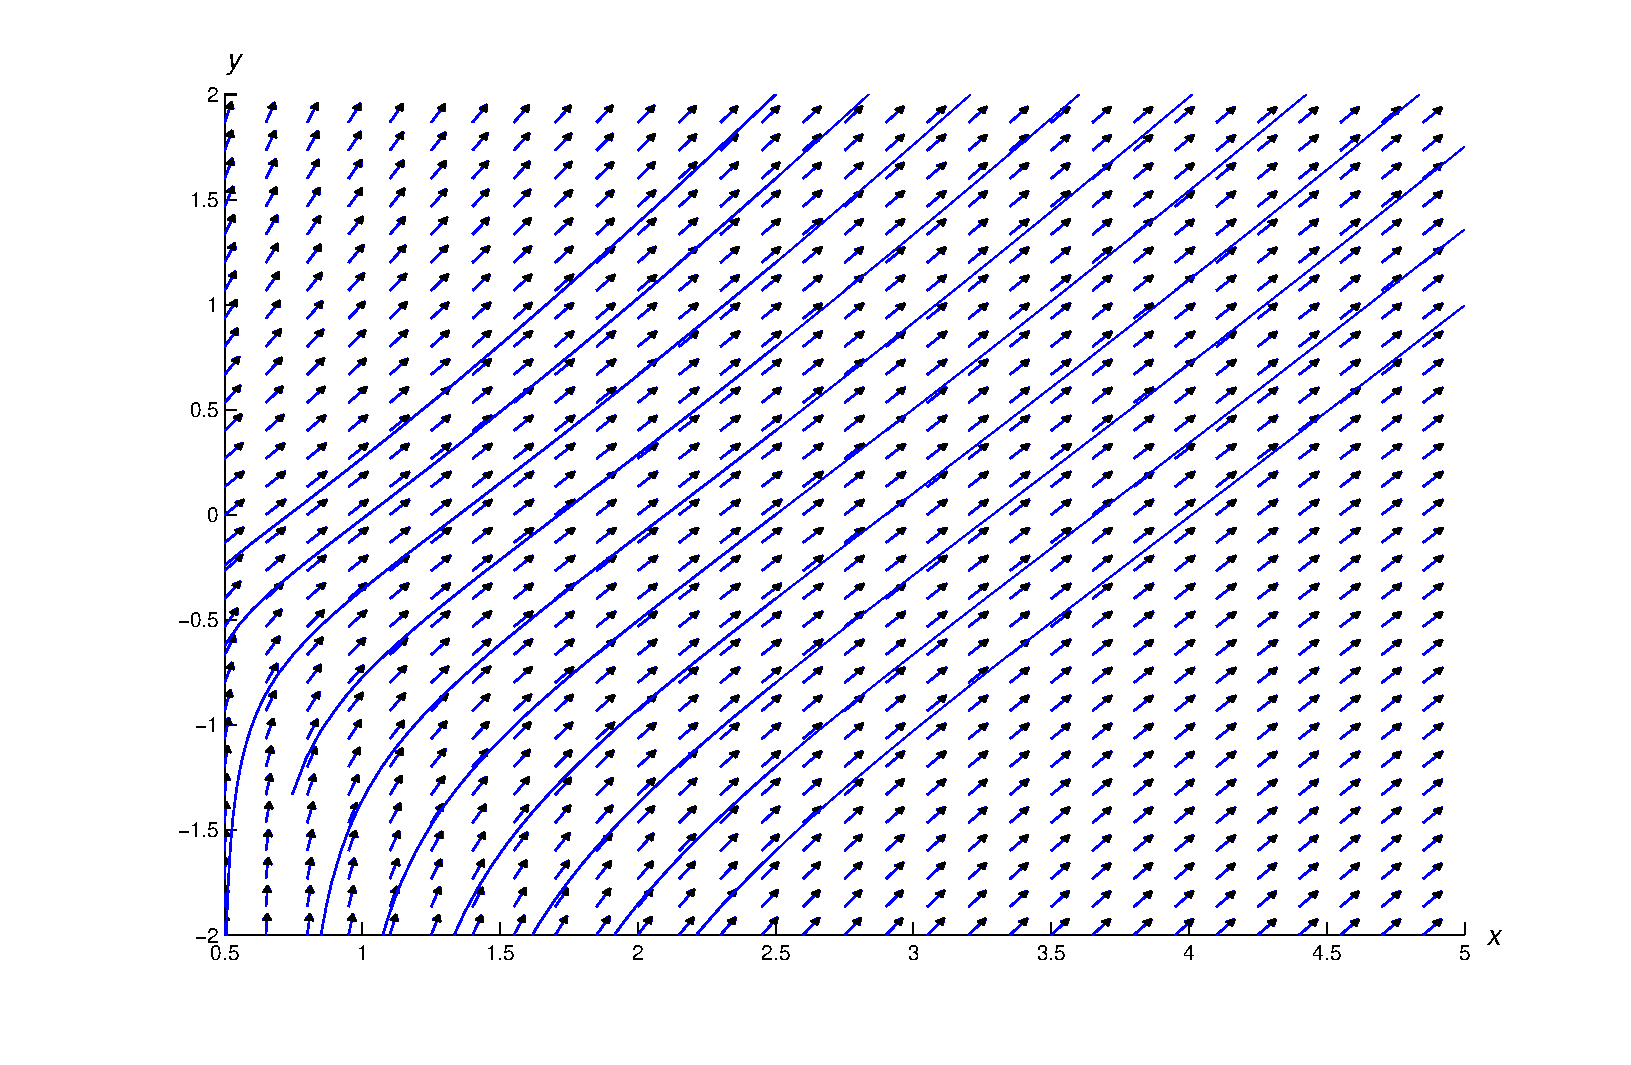
\includegraphics[bb=-78 148 689 643, width=5.67in, height=3.66in, keepaspectratio]{fig020402}
  \color{blue}
  \caption{A direction field and some integral curves for $y'=\dst{\frac{y+xe^{-y/x}}{x}}$}
  \label{figure:2.4.2}
\end{figure}

\begin{example}
  \label{example:2.4.3}\rm \mbox{}
  \newline
  \begin{alist}
    \item % (a)
    Solve
    \begin{equation}
      \label{eq:2.4.9}x^{2}y'=y^{2}+xy-x^{2}.
    \end{equation}

    \item % (b)
    Solve the initial value problem
    \begin{equation}
      \label{eq:2.4.10}x^{2}y'=y^{2}+xy-x^{2},\quad y(1)=2.
    \end{equation}
  \end{alist}
\end{example}

\solutionpart{a} We first find solutions of \eqref{eq:2.4.9} on open intervals that don't contain $x=0$. We can rewrite \eqref{eq:2.4.9} as
\[
  y'=\frac{y^{2}+xy-x^{2}}{x^{2}}
\]
for $x$ in any such interval. Substituting $y=ux$ yields
\[
  u'x+u=\frac{(ux)^{2}+x(ux)-x^{2}}{x^{2}}=u^{2}+u-1,
\]
so
\begin{equation}
  \label{eq:2.4.11}u'x=u^{2}-1.
\end{equation}
By inspection this equation has the constant solutions $u\equiv1$ and $u\equiv-1$. Therefore $y=x$ and $y=-x$ are solutions of \eqref{eq:2.4.9}. If $u$ is a solution of \eqref{eq:2.4.11} that doesn't assume the values $\pm1$ on some interval, separating variables yields
\[
  \frac{u'}{u^{2}-1}=\frac{1}{x},
\]
or, after a partial fraction expansion,
\[
  \frac{1}{2}\left[\frac{1}{u-1}-\frac{1}{u+1}\right]u'= \frac{1}{x}.
\]
Multiplying by 2 and integrating yields
\[
  \ln\left|\frac{u-1}{u+1}\right|=2\ln|x|+k,
\]
or
\[
  \left|\frac{u-1}{u+1}\right|=e^{k}x^{2},
\]
which holds if
\begin{equation}
  \label{eq:2.4.12}\frac{u-1}{u+1}=cx^{2}
\end{equation}
where $c$ is an arbitrary constant. Solving for $u$ yields
\[
  u=\frac{1+cx^{2}}{1-cx^{2}}.
\]

\begin{figure}[htbp]
  \color{blue}
  \begin{minipage}[b]{0.5\linewidth}
    \centering
    \scalebox{.6}{
    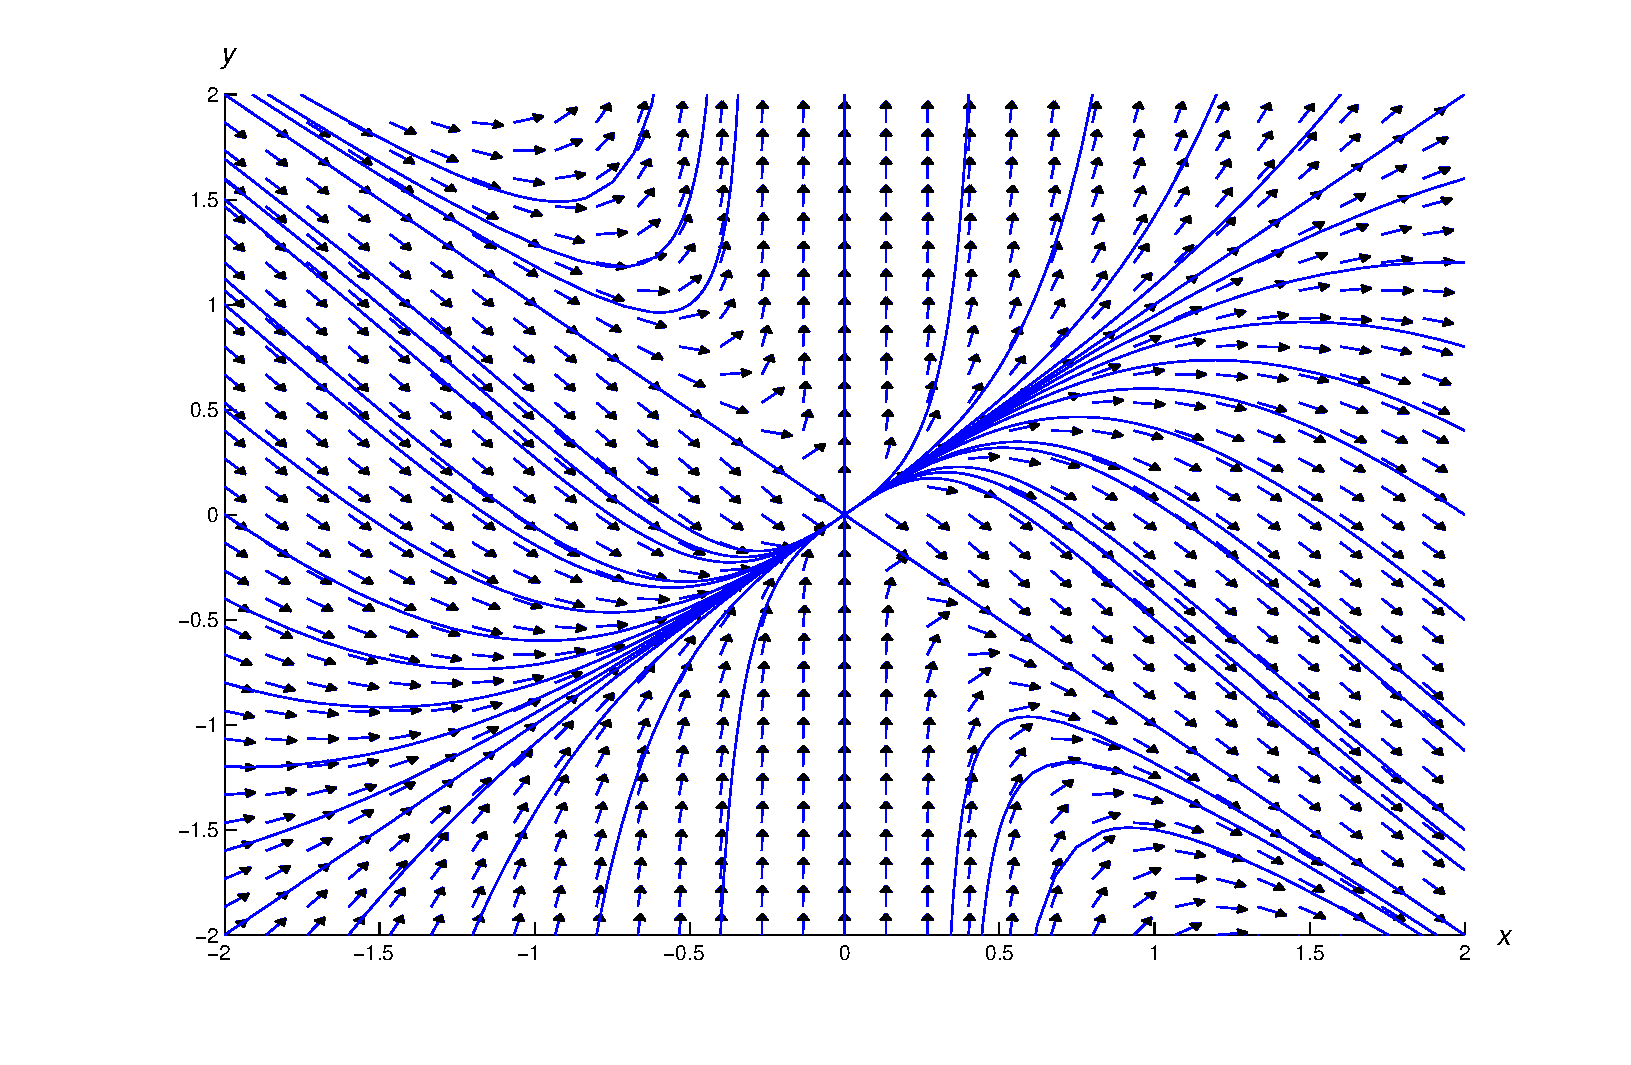
\includegraphics[bb=-78 148 689 643, width=5.67in, height=3.66in, keepaspectratio]{fig020403}
    }
    \color{blue}
    \caption{A direction field and integral curves for $x^{2}y'=y^{2}+xy-x^{2}$}
    \label{figure:2.4.3}
  \end{minipage}
  \hspace{0.6cm}
  \begin{minipage}[b]{0.5\linewidth}
    \centering
    \scalebox{.7}{
    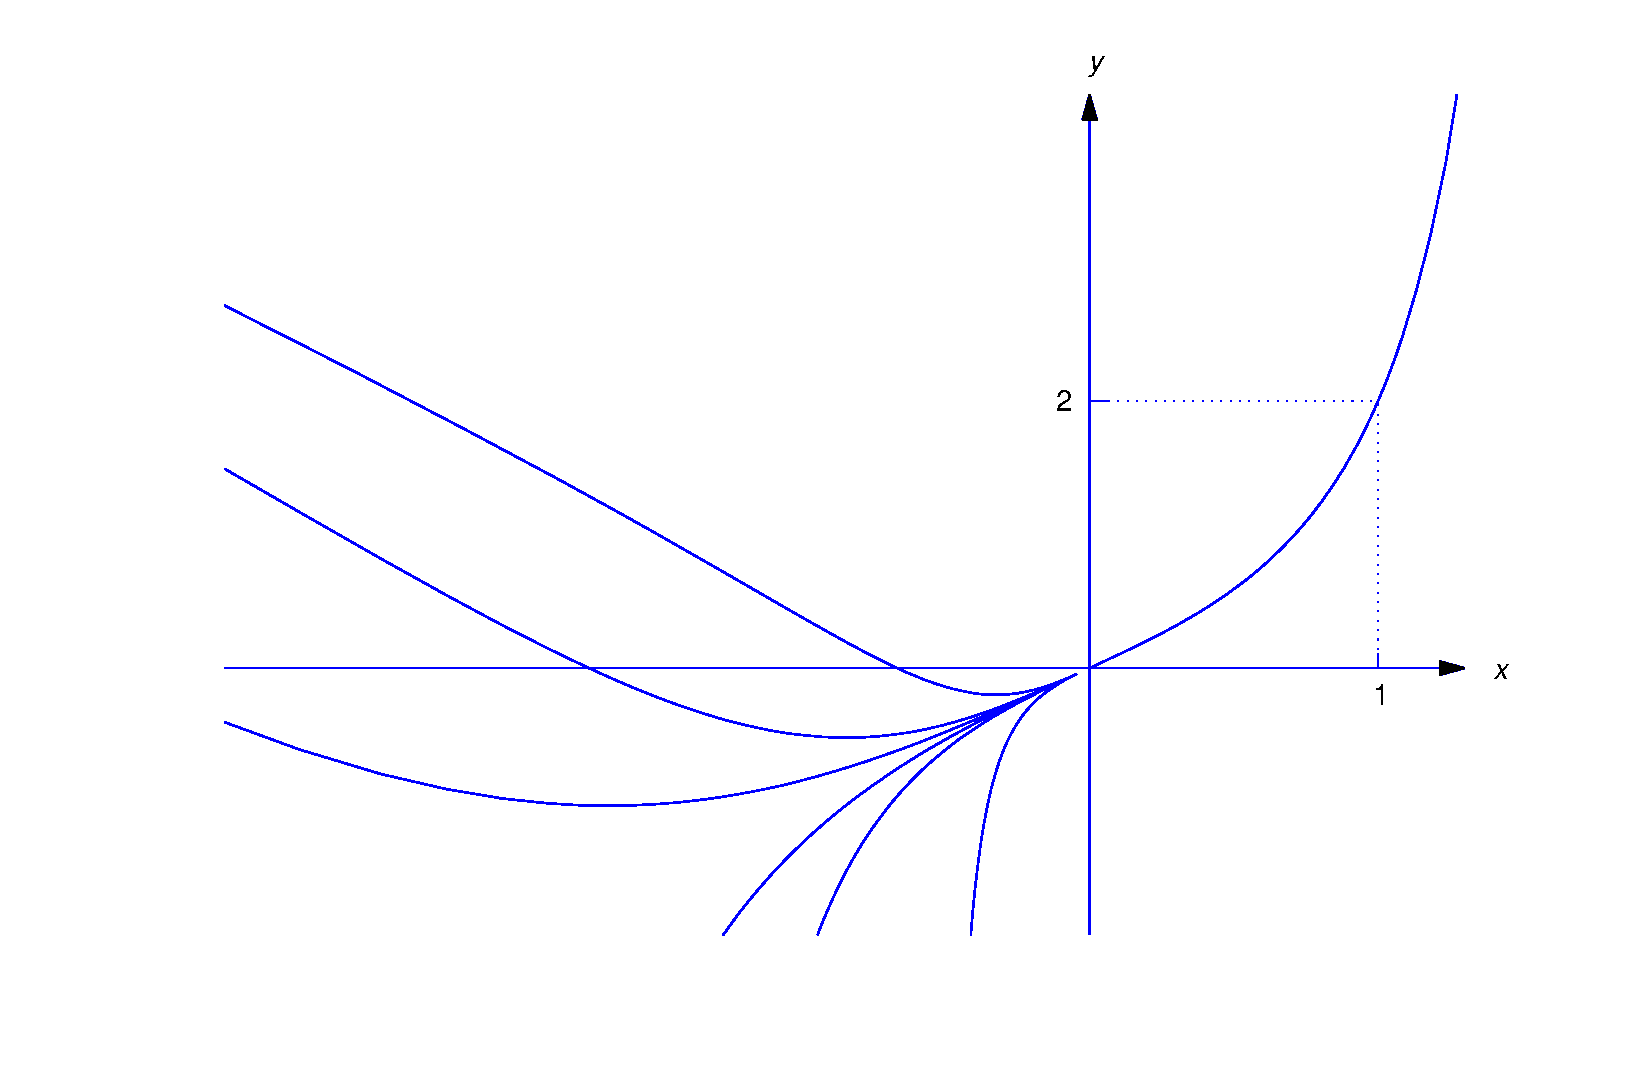
\includegraphics[bb=-78 148 689 643, width=5.67in, height=3.66in, keepaspectratio]{fig020404}}
    \caption{Solutions of $x^{2}y'=y^{2}+xy-x^{2}$,\; $y(1)=2$}
    \label{figure:2.4.4}
  \end{minipage}
\end{figure}

\noindent
Therefore
\begin{equation}
  \label{eq:2.4.13}y=ux=\frac{x(1+cx^{2})}{1-cx^{2}}
\end{equation}
is a solution of \eqref{eq:2.4.10} for any choice of the constant $c$. Setting $c=0$ in \eqref{eq:2.4.13} yields the solution $y=x$. However, the solution $y=-x$ can't be obtained from \eqref{eq:2.4.13}. Thus, the solutions of \eqref{eq:2.4.9} on intervals that don't contain $x=0$ are $y=-x$ and functions of the form \eqref{eq:2.4.13}.

The situation is more complicated if $x=0$ is the open interval. First, note that $y=-x$ satisfies \eqref{eq:2.4.9} on $(-\infty,\infty)$. If $c_{1}$ and $c_{2}$ are arbitrary constants, the function
\begin{equation}
  \label{eq:2.4.14}y=\left\{
  \begin{array}{ll}
    \dst\frac{x(1+c_{1}x^{2})}{1-c_{1}x^{2}},        & a<x<0,    \\
    [2\jot]\dst\frac{x(1+c_{2}x^{2})}{1-c_{2}x^{2}}, & 0\le x<b,
  \end{array}\right.
\end{equation}
is a solution of \eqref{eq:2.4.9} on $(a,b)$, where
\[
  a=\left\{
  \begin{array}{cl}
    -\dst\frac{1}{\sqrt{c_{1}}} & \mbox{ if }c_{1}>0,   \\
    -\infty                     & \mbox{ if }c_{1}\le0,
  \end{array}\right.\mbox{\quad and \quad}b=\left\{
  \begin{array}{cl}
    \dst\frac{1}{\sqrt{c_{2}}} & \mbox{ if }c_{2}>0,   \\
    \infty                     & \mbox{ if }c_{2}\le0.
  \end{array}\right.
\]
We leave it to you to verify this. To do so, note that if $y$ is any function of the form \eqref{eq:2.4.13} then $y(0)=0$ and $y'(0)=1$.

Figure~\ref{figure:2.4.3} shows a direction field and some integral curves for \eqref{eq:2.4.9}.

\solutionpart{b} We could obtain $c$ by imposing the initial condition $y(1)=2$ in \eqref{eq:2.4.13}, and then solving for $c$. However, it's easier to use \eqref{eq:2.4.12}. Since $u=y/x$, the initial condition $y(1)=2$ implies that $u(1)=2$. Substituting this into \eqref{eq:2.4.12} yields $c=1/3$. Hence, the solution of \eqref{eq:2.4.10} is
\[
  y=\frac{x(1+x^{2}/3)}{1-x^{2}/3}.
\]
The interval of validity of this solution is $(-\sqrt{3},\sqrt{3})$. However, the largest interval on which \eqref{eq:2.4.10} has a unique solution is $(0,\sqrt{3})$. To see this, note from \eqref{eq:2.4.14} that any function of the form
\begin{equation}
  \label{eq:2.4.15}y=\left\{
  \begin{array}{ll}
    \dst\frac{x(1+cx^{2})}{1-cx^{2}},   & a<x\le0,         \\[2\jot]
    \dst\frac{x(1+x^{2}/3)}{1-x^{2}/3}, & 0\le x<\sqrt{3},
  \end{array}\right.
\end{equation}
is a solution of \eqref{eq:2.4.10} on $(a,\sqrt{3})$, where $a=-1/\sqrt{c}$ if $c>0$ or $a=-\infty$ if $c\le0$. (Why doesn't this contradict Theorem~\ref{thmtype:2.3.1}?)

Figure~\ref{figure:2.4.4} shows several solutions of the initial value problem~\eqref{eq:2.4.10}. Note that these solutions coincide on $(0,\sqrt{3})$.

In the last two examples we were able to solve the given equations explicitly. However, this isn't always possible, as you'll see in the exercises.

\exercises In Exercises~\ref{exer:2.4.1}--\ref{exer:2.4.4} solve the given Bernoulli equation.

\begin{exerciselist}
  \begin{tabular}[t]{@{}p{168pt}@{}p{168pt}}
    \item\label{exer:2.4.1} $y'+y=y^{2}$ &
    \item\label{exer:2.4.2} $\dst{7xy'-2y=-\frac{x^{2}}{y^{6}}}$
  \end{tabular}

  \begin{tabular}[t]{@{}p{168pt}@{}p{168pt}}
    \item\label{exer:2.4.3} $x^{2}y'+2y=2e^{1/x}y^{1/2}$ &

    \item\label{exer:2.4.4} \vspace*{-5pt}$\dst{(1+x^{2})y'+2xy =\frac{1}{(1+x^{2})y}}$
  \end{tabular}

  \exercisetext{In Exercises~\ref{exer:2.4.5} and \ref{exer:2.4.6} find all solutions. Also, plot a direction field and some integral curves on the indicated rectangular region.}

  \item\label{exer:2.4.5} \CGex $y'-xy=x^{3}y^{3};\quad\{-3\le x\le3,\-2\le y\ge2\}$

  \item\label{exer:2.4.6} \CGex $\dst{y'-\frac{1+x}{3x}y=y^{4}};\quad\{-2\le x\le2,-2\le y\le2\}$

  \exercisetext{In Exercises~\ref{exer:2.4.7}--\ref{exer:2.4.11} solve the initial value problem.}

  \item\label{exer:2.4.7} $y'-2y=xy^{3},\quad y(0)=2\sqrt{2}$

  \item\label{exer:2.4.8} $y'-xy=xy^{3/2},\quad y(1)=4$

  \item\label{exer:2.4.9} $xy'+y=x^{4}y^{4},\quad y(1)=1/2$

  \item\label{exer:2.4.10} $y'-2y=2y^{1/2},\quad y(0)=1$

  \item\label{exer:2.4.11} $\dst{y'-4y=\frac{48x}{y^{2}},\quad y(0)=1}$

  \exercisetext{In Exercises~\ref{exer:2.4.12} and \ref{exer:2.4.13} solve the initial value problem and graph the solution.}

  \item\label{exer:2.4.12} \CGex $x^{2}y'+2xy=y^{3},\quad y(1)=1/\sqrt{2}$

  \item\label{exer:2.4.13} \CGex $y'-y=xy^{1/2},\quad y(0)=4$

  \item\label{exer:2.4.14} You may have noticed that the logistic equation
  \[
    P'=aP(1-\alpha P)
  \]
  from Verhulst's model for population growth can be written in Bernoulli form as
  \[
    P'-aP=-a\alpha P^{2}.
  \]
  This isn't particularly interesting, since the logistic equation is separable, and therefore solvable by the method studied in Section~2.2. So let's consider a more complicated model, where $a$ is a positive constant and $\alpha$ is a positive continuous function of $t$ on $[0,\infty)$. The equation for this model is
  \[
    P'-aP=-a\alpha(t)P^{2},
  \]
  a non-separable Bernoulli equation.
  \begin{alist}
    \item % (a)
    Assuming that $P(0)=P_{0}>0$, find $P$ for $t>0$. \hint{Express your result in terms of the integral $\int_{0}^{t}\alpha(\tau)e^{a\tau}\,d\tau$.}

    \item % (b)
    Verify that your result reduces to the known results for the Malthusian model where $\alpha=0$, and the Verhulst model where $\alpha$ is a nonzero constant.

    \item % (c)
    Assuming that
    \[
      \lim_{t\to\infty}e^{-at}\int_{0}^{t}\alpha(\tau)e^{a\tau}\,d\tau=L
    \]
    exists (finite or infinite), find $\lim_{t\to\infty}P(t)$.
  \end{alist}

  \exercisetext{In Exercises~\ref{exer:2.4.15}--\ref{exer:2.4.18} solve the equation explicitly.}

  \begin{tabular}[t]{@{}p{168pt}@{}p{168pt}}
    \item\label{exer:2.4.15} $y'=\dst\frac{y+x}{x}$ & \vspace*{5pt}
    \item\label{exer:2.4.16} $y'=\dst\frac{y^{2}+2xy}{x^{2}}$
  \end{tabular}

  \begin{tabular}[t]{@{}p{168pt}@{}p{168pt}}
    \item\label{exer:2.4.17} $xy^{3}y'=y^{4}+x^{4}$ &
    \item\label{exer:2.4.18} $y'=\dst\frac{y}{x}+\sec\frac{y}{x}$
  \end{tabular}

  \exercisetext{In Exercises~\ref{exer:2.4.19}-\ref{exer:2.4.21} solve the equation explicitly. Also, plot a direction field and some integral curves on the indicated rectangular region.}

  \item\label{exer:2.4.19} \CGex $x^{2}y'=xy+x^{2}+y^{2};\quad\{-8\le x\le8,-8\le y\le8\}$

  \item\label{exer:2.4.20} \CGex $xyy'=x^{2}+2y^{2};\quad\{-4\le x\le4,-4\le y\le4\}$

  \item\label{exer:2.4.21} \CGex $y'=\dst\frac{2y^{2}+x^{2}e^{-(y/x)^{2}}}{2xy}; \quad\{-8\le x\le8,-8\le y\le8\}$

  \exercisetext{In Exercises~\ref{exer:2.4.22}--\ref{exer:2.4.27} solve the initial value problem.}

  \item\label{exer:2.4.22} $y'=\dst\frac{xy+y^{2}}{x^{2}}, \quad y(-1)=2$

  \item\label{exer:2.4.23} $y'=\dst\frac{x^{3}+y^{3}}{xy^{2}},\quad y(1)=3$

  \item\label{exer:2.4.24} $xyy'+x^{2}+y^{2}=0,\quad y(1)=2$

  \item\label{exer:2.4.25} $y'=\dst\frac{y^{2}-3xy-5x^{2}}{x^{2}},\quad y(1)=-1$

  \item\label{exer:2.4.26} $x^{2}y'=2x^{2}+y^{2}+4xy,\quad y(1)=1$

  \item\label{exer:2.4.27} $xyy'=3x^{2}+4y^{2},\quad y(1)=\sqrt{3}$

  \exercisetext{In Exercises~\ref{exer:2.4.28}--\ref{exer:2.4.34} solve the given homogeneous equation implicitly.}

  \begin{tabular}[t]{@{}p{168pt}@{}p{168pt}}
    \item\label{exer:2.4.28} $y'=\dst\frac{x+y}{x-y}$ &
    \item\label{exer:2.4.29}\vspace*{13pt} $(y'x-y)(\ln|y|-\ln|x|)=x$
  \end{tabular}

  \begin{tabular}[t]{@{}p{168pt}@{}p{168pt}}
    \item\label{exer:2.4.30} $y'=\dst\frac{y^{3}+2xy^{2}+x^{2}y+x^{3}}{x(y+x)^{2}}$ &
    \item\label{exer:2.4.31} $y'=\dst\frac{x+2y}{2x+y}$
  \end{tabular}

  \begin{tabular}[t]{@{}p{168pt}@{}p{168pt}}
    \item\label{exer:2.4.32} $y'=\dst\frac{y}{y-2x}$ &
    \item\label{exer:2.4.33} $y'=\dst\frac{xy^{2}+2y^{3}}{x^{3}+x^{2}y+xy^{2}}$
  \end{tabular}

  \item\label{exer:2.4.34} $y'=\dst\frac{x^{3}+x^{2}y+3y^{3}}{x^{3}+3xy^{2}}$

  \item\label{exer:2.4.35} \Lex
  \begin{alist}
    \item % (a)
    Find a solution of the initial value problem
    \[
      x^{2}y'=y^{2}+xy-4x^{2},\quad y(-1)=0 \eqno{\rm(A)}
    \]
    on the interval $(-\infty,0)$. Verify that this solution is actually valid on $(-\infty,\infty)$.

    \item % (b)
    Use Theorem~\ref{thmtype:2.3.1} to show that (A) has a unique solution on $(-\infty,0)$.

    \item % (c)
    Plot a direction field for the differential equation in (A) on a square
    \[
      \{-r\le x\le r,-r\le y\le r\},
    \]
    where $r$ is any positive number. Graph the solution you obtained in \part{a} on this field.

    \item % (d)
    Graph other solutions of (A) that are defined on $(-\infty,\infty)$.

    \item % (e)
    Graph other solutions of (A) that are defined only on intervals of the form $(-\infty,a)$, where is a finite positive number.
  \end{alist}

  \item\label{exer:2.4.36} \Lex
  \begin{alist}
    \item % (a)
    Solve the equation
    \[
      xyy'=x^{2}-xy+y^{2}\eqno{\rm(A)}
    \]
    implicitly.

    \item % (b)
    Plot a direction field for (A) on a square
    \[
      \{0\le x\le r,0\le y\le r\}
    \]
    where $r$ is any positive number.

    \item % (c)
    Let $K$ be a positive integer. (You may have to try several choices for $K$.) Graph solutions of the initial value problems
    \[
      xyy'=x^{2}-xy+y^{2},\quad y(r/2)=\frac{kr}{K},
    \]
    for $k=1$, $2$, \dots, $K$. Based on your observations, find conditions on the positive numbers $x_{0}$ and $y_{0}$ such that the initial value problem
    \[
      xyy'=x^{2}-xy+y^{2},\quad y(x_{0})=y_{0}, \eqno{\rm(B)}
    \]
    has a unique solution (i) on $(0,\infty)$ or (ii) only on an interval $(a,\infty)$, where $a>0$?

    \item % (d)
    What can you say about the graph of the solution of (B) as $x\to\infty$? (Again, assume that $x_{0}>0$ and $y_{0}>0$.)
  \end{alist}

  \item\label{exer:2.4.37} \Lex
  \begin{alist}
    \item % (a)
    Solve the equation
    \[
      y'=\frac{2y^{2}-xy+2x^{2}}{xy+2x^{2}}\eqno{\rm(A)}
    \]
    implicitly.

    \item % (b)
    Plot a direction field for (A) on a square
    \[
      \{-r\le x\le r,-r\le y\le r\}
    \]
    where $r$ is any positive number. By graphing solutions of (A), determine necessary and sufficient conditions on $(x_{0},y_{0})$ such that (A) has a solution on (i) $(-\infty,0)$ or (ii) $(0,\infty)$ such that $y(x_{0})=y_{0}$.
  \end{alist}

  \item\label{exer:2.4.38} \Lex Follow the instructions of Exercise~\ref{exer:2.4.37} for the equation
  \[
    y'=\frac{xy+x^{2}+y^{2}}{xy}.
  \]

  \item\label{exer:2.4.39} \Lex Pick any nonlinear homogeneous equation $y'=q(y/x)$ you like, and plot direction fields on the square $\{-r\le x\le r,\ -r\le y\le r\}$, where $r>0$. What happens to the direction field as you vary $r$? Why?

  \item\label{exer:2.4.40} Prove: If $ad-bc\ne0$, the equation
  \[
    y'=\frac{ax+by+\alpha}{cx+dy+\beta}
  \]
  can be transformed into the homogeneous nonlinear equation
  \[
    \frac{dY}{dX}=\frac{aX+bY}{cX+dY}
  \]
  by the substitution $x=X-X_{0}$, $y=Y-Y_{0}$, where $X_{0}$ and $Y_{0}$ are suitably chosen constants.

  \exercisetext{In Exercises~\ref{exer:2.4.41}-\ref{exer:2.4.43} use a method suggested by Exercise~\ref{exer:2.4.40} to solve the given equation implicitly.}

  \begin{tabular}[t]{@{}p{168pt}@{}p{168pt}}
    \item\label{exer:2.4.41} $y'=\dst\frac{-6x+y-3}{2x-y-1}$ &
    \item\label{exer:2.4.42}\vspace*{10pt} $y'=\dst\frac{2x+y+1}{x+2y-4}$
  \end{tabular}

  \item\label{exer:2.4.43} $y'=\dst\frac{-x+3y-14}{x+y-2}$

  \exercisetext{In Exercises~\ref{exer:2.4.44}--\ref{exer:2.4.51} find a function $y_{1}$ such that the substitution $y=uy_{1}$ transforms the given equation into a separable equation of the form \eqref{eq:2.4.6}. Then solve the given equation explicitly.}

  \begin{tabular}[t]{@{}p{168pt}@{}p{168pt}}
    \item\label{exer:2.4.44} $3xy^{2}y'=y^{3}+x$ & \vspace*{10pt}
    \item\label{exer:2.4.45} $xyy'=3x^{6}+6y^{2}$
  \end{tabular}

  \begin{tabular}[t]{@{}p{168pt}@{}p{168pt}}
    \item\label{exer:2.4.46} $x^{3}y'=2(y^{2}+x^{2}y-x^{4})$ &
    \item\label{exer:2.4.47} $y'=y^{2}e^{-x}+4y+2e^{x}$
  \end{tabular}

  \begin{tabular}[t]{@{}p{168pt}@{}p{168pt}}
    \item\label{exer:2.4.48} $y'=\dst\frac{y^{2}+y\tan x+\tan^{2}x}{\sin^{2}x}$ &
    \item\label{exer:2.4.49} $x(\ln x)^{2}y'=-4(\ln x)^{2}+y\ln x+y^{2}$
  \end{tabular}

  \begin{tabular}[t]{@{}p{168pt}@{}p{168pt}}
    \item\label{exer:2.4.50} $2x(y+2\sqrt{x})y'=(y+\sqrt{x})^{2}$ &
    \item\label{exer:2.4.51} $(y+e^{x^{2}})y'=2x(y^{2}+ye^{x^{2}}+e^{2x^{2}})$
  \end{tabular}

  \medskip

  \item\label{exer:2.4.52} Solve the initial value problem
  \[
    y'+\frac{2}{x}y=\frac{3x^{2}y^{2}+6xy+2}{x^{2}(2xy+3)},\quad y(2)=2.
  \]

  \item\label{exer:2.4.53} Solve the initial value problem
  \[
    y'+\frac{3}{x}y=\frac{3x^{4}y^{2}+10x^{2}y+6}{x^{3}(2x^{2}y+5)},\quad y(1)=1.
  \]

  \item\label{exer:2.4.54} Prove: If $y$ is a solution of a homogeneous nonlinear equation $y'=q(y/x)$, so is $y_{1}=y(ax)/a$, where $a$ is any nonzero constant.

  \item\label{exer:2.4.55} A {\color{blue}\it generalized}
  \href{https://mathshistory.st-andrews.ac.uk/Biographies/Riccati/}{\color{blue}
  \it Riccati equation}
  is of the form
  \[
    y'=P(x)+Q(x)y+R(x)y^{2}. \eqno{\rm(A)}
  \]
  (If $R\equiv-1$, (A) is a
  \href{https://mathshistory.st-andrews.ac.uk/Biographies/Riccati/}{\color{blue}
  \it Riccati equation\/}.) Let $y_{1}$ be a known solution and $y$ an arbitrary solution of (A). Let $z=y-y_{1}$. Show that $z$ is a solution of a Bernoulli equation with $n=2$.

  \exercisetext{In Exercises~\ref{exer:2.4.56}--\ref{exer:2.4.59}, given that $y_{1}$ is a solution of the given equation, use the method suggested by Exercise \ref{exer:2.4.55} to find other solutions.}

  \item\label{exer:2.4.56} $y'=1+x-(1+2x)y+xy^{2}$; \quad $y_{1}=1$

  \item\label{exer:2.4.57} $y'=e^{2x}+(1-2e^{x})y+y^{2}$; \quad $y_{1}=e^{x}$

  \item\label{exer:2.4.58} $xy'=2-x+(2x-2)y-xy^{2}$; \quad $y_{1}=1$

  \item\label{exer:2.4.59} $xy'=x^{3}+(1-2x^{2})y+xy^{2}$; \quad $y_{1}=x$
\end{exerciselist}
